% sections/03_mems.tex  (owner: mems)
% Code:    code/mems_symbolic_checks.py   (sympy: every formula below)
%          code/mems_profiles_shooting.py (self-similar profiles, Fig. mems_profile_shooting)
%          code/mems_spectrum_numerics.py (collocation spectra, Fig. mems_spectrum)
%          code/mems_damped_ode.py        (damped ODE asymptotics, pull-in values)
% Bib:     bib/mems.bib (new keys) + keys from bib/lit.bib, bib/lead.bib
\section{Hyperbolic MEMS: stability of self-similar touchdown}
\label{mems:sec}

This section carries out the programme of \cref{fw:sec} for the inertial
MEMS model \eqref{lit:eq:memsq} in full, including the points where the
singular nonlinearity and the \emph{negative} scaling exponent $s=-\sigma$
require extra care. Throughout, the MEMS (voltage) parameter is called
$\lambda$, as in the engineering literature, and the \emph{spectral parameter}
is called $\mu$ (it is called $\lambda$ in \cref{fw:sec}).

\begin{table}[ht]
\centering\small
\begin{tabular}{@{}p{0.50\textwidth}p{0.19\textwidth}p{0.23\textwidth}@{}}
\toprule
\raggedright Statement & \raggedright Where & \raggedright Status \tabularnewline
\midrule
\raggedright ODE touchdown $w=c(T-t)^{2/(q+1)}$, Lorentz family, energy expansion & \raggedright \cref{mems:prop-ode,mems:lem-sym} & \raggedright elementary/known \tabularnewline
\raggedright $d=1$: every smooth positive self-similar profile is a boosted ODE profile & \raggedright \cref{mems:thm-d1} & \raggedright proved here \tabularnewline
\raggedright $d=2,3$: a sequence of non-trivial profiles $\psi_n\to A|\xi|^\sigma$ & \raggedright \cref{mems:tab-prof,mems:conj-prof} & \raggedright numerical; conjecture \tabularnewline
\raggedright Spectrum at the ODE profile, gap $\omega_0=\min\{1,\frac{2(q-1)}{q+1}\}$ & \raggedright \cref{mems:prop-spec} & \raggedright proved here \tabularnewline
\raggedright No Jordan chains at $\mu=1,0$; Jordan block at $\mu=-1$ if $q=3$ & \raggedright \cref{mems:lem-jordan,mems:rem-q3} & \raggedright proved here ($d\le3$) \tabularnewline
\raggedright Free operator: dissipative up to finite rank on $H^k\times H^{k-1}$ & \raggedright \cref{mems:lem-free} & \raggedright proved here \tabularnewline
\raggedright Nonlinear stability modulo time translation and boosts & \raggedright \cref{mems:thm-main} & \raggedright proof sketch \tabularnewline
\raggedright Damping $\gamma w_t$ (radial \emph{and} nonradial) & \raggedright \cref{mems:prop-damped,mems:cor-damped} & \raggedright proof sketch \tabularnewline
\raggedright Excited profiles have extra unstable modes & \raggedright \cref{mems:sec-num} & \raggedright numerical only \tabularnewline
\bottomrule

\end{tabular}
\caption{Results of \cref{mems:sec}. ``Proof sketch'' means all
estimates are indicated and the argument follows
\cite{DonningerSchoerkhuber2016,DonningerSchoerkhuber2017,Ostermann2024}, but
not every detail has been written out.}
\label{mems:tab-status}
\end{table}

\subsection{The model}
\label{mems:sec-model}
In the small-aspect-ratio limit the deflection $u$ of an electrostatically
actuated membrane over a ground plate satisfies $\varepsilon^2u_{tt}+\gamma
u_t-\Delta u=-\lambda f(x)(1+u)^{-2}$ in $\Omega$, $u=0$ on $\partial\Omega$
\cite{PeleskoBernstein2002,FloresEtAl2007,EspositoGhoussoubGuo2010}; see
\cref{lit:mems} for the variants. For the gap $w=1+u\in(0,1]$, in the inertial
time $t/\varepsilon$ (and writing again $t$, $\gamma$ for $t/\varepsilon$,
$\gamma/\varepsilon$), and allowing the force laws $w^{-q}$ ($q=2$ Coulomb,
$q=3$ van der Waals, $q=4$ Casimir), we study
\begin{equation}\label{mems:eq}
  w_{tt}+\gamma w_t-\Delta w=-\lambda\,w^{-q},\qquad q>1,\ \lambda>0,\ \gamma\ge0 .
\end{equation}
\emph{Touchdown} (quenching) at $(T,x_0)$ means $w(t,x)\to0$ as $(t,x)\to(T,x_0)$;
then $\partial_tw\to-\infty$ (infinite impact speed, see below). We put
\[
  \sigma:=\frac{2}{q+1}\in(0,1),\qquad
  c^{q+1}:=\frac{\lambda}{\sigma(1-\sigma)}=\frac{\lambda(q+1)^2}{2(q-1)}
  \qquad(q=2:\ \sigma=\tfrac23,\ c=(9\lambda/2)^{1/3}),
\]
so $c=\kappa_q$ in \eqref{lit:eq:memsode}. Two scalings will be used: if $w$
solves \eqref{mems:eq} with damping $\gamma$, then $\mu_0^{-\sigma}w(\mu_0
t,\mu_0 x)$ solves it with damping $\mu_0\gamma$ (so only $\gamma T$ is
scale-invariant), and $\lambda^{-1/(q+1)}w$ solves it with $\lambda=1$ (used in
the numerics; it changes the boundary value $w|_{\partial\Omega}=1$, which is
irrelevant for the local analysis).

\subsection{ODE touchdown and its symmetry orbit}
\label{mems:sec-ode}

\begin{proposition}[ODE touchdown]\label{mems:prop-ode}
Let $\gamma=0$ and let $W>0$ solve $W''=-\lambda W^{-q}$ on $[0,T)$ with
$W(t)\to0$ as $t\to T$. Let $E=\tfrac12W'^2+\lambda W^{1-q}/(1-q)$ (conserved;
$E=\tfrac12 W'^2+\lambda\log W$ if $q=1$).
\begin{enumerate}[label=(\roman*),nosep]
\item If $q>1$, then with $\theta=T-t$,
  $W=c\,\theta^{\sigma}\big(1+e\,\theta^{2-2\sigma}+O(\theta^{4-4\sigma})\big)$,
  $e=E/(c^2\sigma(3-2\sigma))$, and $W'=-c\sigma\theta^{\sigma-1}(1+o(1))\to-\infty$.
  The exact power law $c(T-t)^\sigma$ is the zero-energy solution.
\item If $0<q<1$, touchdown occurs with finite speed, $W'(T)=-\sqrt{2E}$; if
  $q=1$, $W=\theta\sqrt{2\lambda\log(1/\theta)}\,(1+o(1))$. In both cases there is
  no solution $c\,\theta^{\sigma}$ with $\sigma<1$ (indeed $\sigma\ge1$ forces
  $\sigma(1-\sigma)\le0$), i.e.\ $q>1$ is exactly the condition $s=-\sigma>-1$
  of \cref{fw:thm-spec}.
\item Released from rest, $W(0)=1$, $W'(0)=0$, the touchdown time is
  $T_0=\int_0^1\big(\tfrac{2\lambda}{q-1}(W^{1-q}-1)\big)^{-1/2}dW$, e.g.\
  $T_0=\pi/(2\sqrt{2\lambda})$ for $q=2$ and $T_0=\lambda^{-1/2}$ for $q=3$.
\end{enumerate}
\end{proposition}

\begin{proof}
(i) $W'<0$ near $T$ and $W'^2=2E+\frac{2\lambda}{q-1}W^{1-q}$, so
$T-t=\int_0^W(2E+\frac{2\lambda}{q-1}V^{1-q})^{-1/2}dV$. Expanding the integrand
for $V\to0$ gives $\theta=\frac{2}{q+1}\sqrt{\frac{q-1}{2\lambda}}\,W^{\frac{q+1}2}
(1+O(W^{q-1}))$, i.e.\ $W^{q+1}=c^{q+1}\theta^2(1+O(\theta^{2-2\sigma}))$
since $\sigma(q-1)=2-2\sigma$; the coefficient $e$ follows by inserting the
ansatz into $E$ (the $\theta^0$-terms give $E=c^2e\,\sigma(3-2\sigma)$). (ii)
For $q<1$ the potential $\lambda W^{1-q}/(1-q)$ vanishes at $W=0$; for $q=1$
it diverges only logarithmically. (iii) Separation of variables. All formulas
are checked in \texttt{mems\_symbolic\_checks.py} and, including $e$,
numerically in \texttt{mems\_damped\_ode.py}.
\end{proof}

\begin{lemma}[Symmetry orbit]\label{mems:lem-sym}
For $T\in\mathbb R$ and $a\in\mathbb R^d$, $|a|<1$,
\begin{equation}\label{mems:boost}
  w^{T,a}(t,x)=c\,(1-|a|^2)^{-\sigma/2}\,(T-t+a\cdot x)^{\sigma}
\end{equation}
solves $w_{tt}-\Delta w=-\lambda w^{-q}$ where $T-t+a\cdot x>0$, in particular in
the backward cone $\Gamma_T$, where $T-t+a\cdot x\ge(1-|a|)(T-t)$. In the
similarity variables of $(T,0)$ it is the static profile
\begin{equation}\label{mems:psia}
  \psi_a(\xi)=c\,(1-|a|^2)^{-\sigma/2}(1+a\cdot\xi)^{\sigma},\qquad
  \psi_a\ge c\Big(\frac{1-|a|}{1+|a|}\Big)^{\sigma/2}>0\ \text{on }\overline{B^d}.
\end{equation}
Space translations act trivially on $w^{T,0}$ and as time translations on
$w^{T,a}$: $w^{T,a}(t,x-x_0)=w^{T-a\cdot x_0,a}(t,x)$.
\end{lemma}

\begin{proof}
With $F=T-t+a\cdot x$, $\partial_t^2F^\sigma-\Delta F^\sigma=-\sigma(1-\sigma)(1-|a|^2)F^{\sigma-2}$,
and $\lambda c^{-q}(1-|a|^2)^{q\sigma/2}F^{-q\sigma}=\sigma(1-\sigma)c\,(1-|a|^2)^{1-\sigma/2}F^{\sigma-2}$
because $q\sigma=2-\sigma$. (Also verified symbolically for $d=3$ and general $a$.)
\end{proof}

The touchdown set of $w^{T,a}$ is the spacelike hyperplane $t=T+a\cdot x$; the
boost parameter is the gradient of the touchdown-time function. Hence the
orbit of the ODE solution under the symmetries is $(d+1)$-dimensional, which
will match the $1+d$ non-negative eigenvalues found in \cref{mems:prop-spec}.

\subsection{Self-similar profiles}
\label{mems:sec-prof}
Inserting $w=(T-t)^{\sigma}\psi(x/(T-t))$ into \eqref{mems:eq} with $\gamma=0$
gives $w_{tt}-\Delta w+\lambda w^{-q}=-(T-t)^{\sigma-2}\mathcal P[\psi]$ with
\begin{equation}\label{mems:profile}
  \mathcal P[\psi]:=(\delta_{ij}-\xi_i\xi_j)\partial_i\partial_j\psi-2(1-\sigma)\Lambda\psi+\sigma(1-\sigma)\psi-\lambda\psi^{-q},
\end{equation}
and for radial $\psi(\rho)$, $\rho=|\xi|$,
\begin{equation}\label{mems:profile-rad}
  (1-\rho^2)\psi''+\Big(\frac{d-1}{\rho}-2(1-\sigma)\rho\Big)\psi'+\sigma(1-\sigma)\psi-\lambda\psi^{-q}=0 .
\end{equation}
At $\rho=1$ the Frobenius exponents are $0$ and $\frac{d-1}2+\sigma$. The
solutions analytic at $\rho=1$ form a one-parameter family $\psi(1)=b$,
$\psi'(1)=(\lambda b^{-q}-\sigma(1-\sigma)b)/(d-3+2\sigma)$, except in the
resonant case $d-3+2\sigma=0$, i.e.\ $(d,q)=(2,3)$, where analyticity
\emph{forces} $\psi(1)=c$ and $\psi'(1)$ is free. At $\rho=0$ the regular
solutions are parametrised by $\psi(0)$. Smooth radial profiles are therefore
generically isolated. The constant $\psi\equiv c$ is always one of them; its
boosts $\psi_a$, $a\ne0$, are smooth but not radial.

\begin{theorem}[Classification in $d=1$]\label{mems:thm-d1}
Let $d=1$, $q>1$, and let $\psi\in C^2(-1,1)\cap C^1[-1,1]$ be positive on
$[-1,1]$ with $\mathcal P[\psi]=0$. Then $\psi=\psi_a$ for a unique
$a\in(-1,1)$. In particular $\psi\equiv c$ is the only even profile.
\end{theorem}

\begin{proof}
Use rapidity coordinates in the cone, $T-t=R\cosh\eta$, $x=R\sinh\eta$, so
$\xi=\tanh\eta$ and $w_{tt}-w_{xx}=R^{-1}\partial_R(R\partial_Rw)-R^{-2}\partial_\eta^2w$.
For $w=(T-t)^\sigma\psi(\xi)=R^\sigma\Phi(\eta)$, $\Phi(\eta):=\cosh^\sigma\!\eta\,\psi(\tanh\eta)$,
the profile equation becomes the \emph{autonomous} ODE
$\Phi''=\sigma^2\Phi+\lambda\Phi^{-q}$ on $\mathbb R$, with conserved energy
$E=\frac12\Phi'^2-\frac12\sigma^2\Phi^2+\frac{\lambda}{q-1}\Phi^{1-q}$. In terms of
$\psi$,
\[
  2E=(1-\xi^2)^{1-\sigma}\Big[-\sigma^2\psi^2+2\sigma\xi\psi\psi'+(1-\xi^2)\psi'^2+\tfrac{2\lambda}{q-1}\psi^{1-q}\Big].
\]
The bracket is bounded on $[-1,1]$ because $\psi\in C^1$ and $\psi>0$, and
$1-\sigma>0$; letting $\xi\to1$ gives $E=0$. On $\{E=0\}$,
$\Phi'^2=\sigma^2\Phi^{1-q}(\Phi^{q+1}-c^{q+1})$, so $\Phi\ge c$, and
$\Phi''>0$. If $\Phi'$ had no zero, say $\Phi'>0$, then $\Phi\downarrow L\ge c$
as $\eta\to-\infty$ with $\Phi'\to0$, so $L=c$, but then
$\Phi''\to\sigma^2c+\lambda c^{-q}>0$ contradicts $\Phi'>0$ near $-\infty$.
Hence $\Phi'(\eta_0)=0$, $\Phi(\eta_0)=c$ for some $\eta_0$, and by uniqueness for
the initial value problem $\Phi=c\cosh^\sigma(\eta-\eta_0)$ (this solves the ODE,
\texttt{mems\_symbolic\_checks.py}). Undoing the substitution gives
$\psi=\psi_a$ with $a=-\tanh\eta_0$.
\end{proof}

This is the MEMS analogue of the one-dimensional classification of
Merle and Zaag for power nonlinearities \cite{MerleZaag2007}. The argument
uses the conserved energy of the rapidity ODE and has no direct analogue for
$d\ge2$: the radial equation on hyperbolic space,
$\Phi''+(d-1)\coth\eta\,\Phi'=\sigma(\sigma+d-1)\Phi+\lambda\Phi^{-q}$, only has a
monotone energy, which tends to $-\infty$ for smooth profiles.

\paragraph{Non-trivial profiles for $d\ge2$ (numerical).}
For $d\ge2$, \eqref{mems:profile-rad} has the singular solution
\begin{equation}\label{mems:singular}
  \psi_*(\rho)=A\rho^{\sigma},\qquad A^{q+1}=\frac{\lambda}{\sigma(\sigma+d-2)},
\end{equation}
which is the \emph{static} singular solution $w_*(x)=A|x|^{\sigma}$ of
$\Delta w=\lambda w^{-q}$ (a membrane touching the plate at one point). It is
analytic at $\rho=1$ and singular only at $\rho=0$. Near $\rho=0$, the
linearisation at $\psi_*$ is $\Delta v+q\sigma(\sigma+d-2)|\xi|^{-2}v$, whose
solutions $|\xi|^{-\frac{d-2}2\pm i\nu}$,
\begin{equation}\label{mems:nu}
  \nu^2=q\sigma(\sigma+d-2)-\tfrac{(d-2)^2}4,
\end{equation}
oscillate iff $\nu^2>0$. This Joseph--Lundgren-type condition holds for all
$q>1$ when $d=2,3$, and for $q=2$ exactly when $2\le d\le7$. (To our knowledge this is the same
range $2\le d\le7$ that produces the oscillating bifurcation diagram, with
infinitely many fold points, of the stationary MEMS problem; see
\cite{EspositoGhoussoubGuo2010}.)
% TODO verify: Guo--Wei (2008, J. London Math. Soc.) "infinitely many turning points" for 2<=N<=7.
We solved \eqref{mems:profile-rad} by two-sided shooting (regular series at
$\rho=0$ and $\rho=1$, matched at $\rho=\frac12$; robust under changes of the
matching point; \texttt{mems\_profiles\_shooting.py}), scanning
$\psi(0)\in[10^{-3}c,50c]$ for $d=2,3$ and $\psi(0)\in[0.02c,50c]$ for $d=1$.
\Cref{mems:tab-prof} and \cref{mems:fig-prof} summarise the results.
\begin{itemize}[nosep]
\item $d=1$: only $\psi\equiv c$, as \cref{mems:thm-d1} requires.
\item $d=2,3$, $q=2,3,4$: besides $\psi_0\equiv c$, a sequence of smooth
positive profiles $\psi_1,\psi_2,\dots$ with $\psi_n(0)\downarrow0$, each strictly
increasing in $\rho$, converging to $\psi_*$ away from $\rho=0$ (e.g.\
$\sup_{[1/2,1]}|\psi_3-\psi_*|<10^{-4}c$ for $d=3,q=2$). The ratios
$\psi_n(0)/\psi_{n+1}(0)$ converge to $e^{\sigma\pi/\nu}$. This is what the
heuristic predicts: in the inner region the profile equation reduces to the
scale-invariant static equation, so the inner solutions are rescalings
$\ell^{\sigma}V(\rho/\ell)$ of a single function. Matching their oscillation
$\cos(\nu\log\rho+\varphi)$ about $\psi_*$ with the outer region quantises
$\nu\log\ell$ modulo $\pi$.
\end{itemize}

\begin{table}[ht]
\centering\small
\begin{tabular}{@{}lccccc@{}}
\toprule
$(d,q)$ & $\psi_1(0)/c$ & $\psi_2(0)/c$ & $\psi_3(0)/c$ & observed ratios & $e^{\sigma\pi/\nu}$\\
\midrule
$(2,2)$ & $0.14519$ & $0.015139$ & $0.0016489$ & $9.59,\ 9.18$ & $9.221$\\
$(3,2)$ & $0.24534$ & $0.056547$ & $0.012713$ & $4.34,\ 4.45$ & $4.443$\\
$(2,3)$ & $0.22125$ & $0.033948$ & $0.0055884$ & $6.52,\ 6.07$ & $6.134$\\
$(3,3)$ & $0.36986$ & $0.12232$ & $0.040285$ & $3.024,\ 3.036,\ 3.0365$ & $3.0365$\\
$(2,4)$ & $0.27636$ & $0.053286$ & $0.011243$ & $5.19,\ 4.74,\ 4.83$ & $4.811$\\
$(3,4)$ & $0.45746$ & $0.18697$ & $0.076792$ & $2.447,\ 2.435,\ 2.437$ & $2.437$\\
\bottomrule
\end{tabular}
\caption{Non-trivial smooth radial self-similar profiles ($\psi_0\equiv c$
omitted). Values of $\psi_n(0)/c$ are independent of $\lambda$. The limits
$\psi_n(1)\to A$ are $A/c=0.7937$ $(2,2)$, $0.5848$ $(3,2)$, $1$ $(2,3)$,
$0.7598$ $(3,3)$, $1.0845$ $(2,4)$, $0.8441$ $(3,4)$. Ratios are
consecutive quotients $\psi_n(0)/\psi_{n+1}(0)$, including further members
not listed.}
\label{mems:tab-prof}
\end{table}

\begin{figure}[ht]
\centering
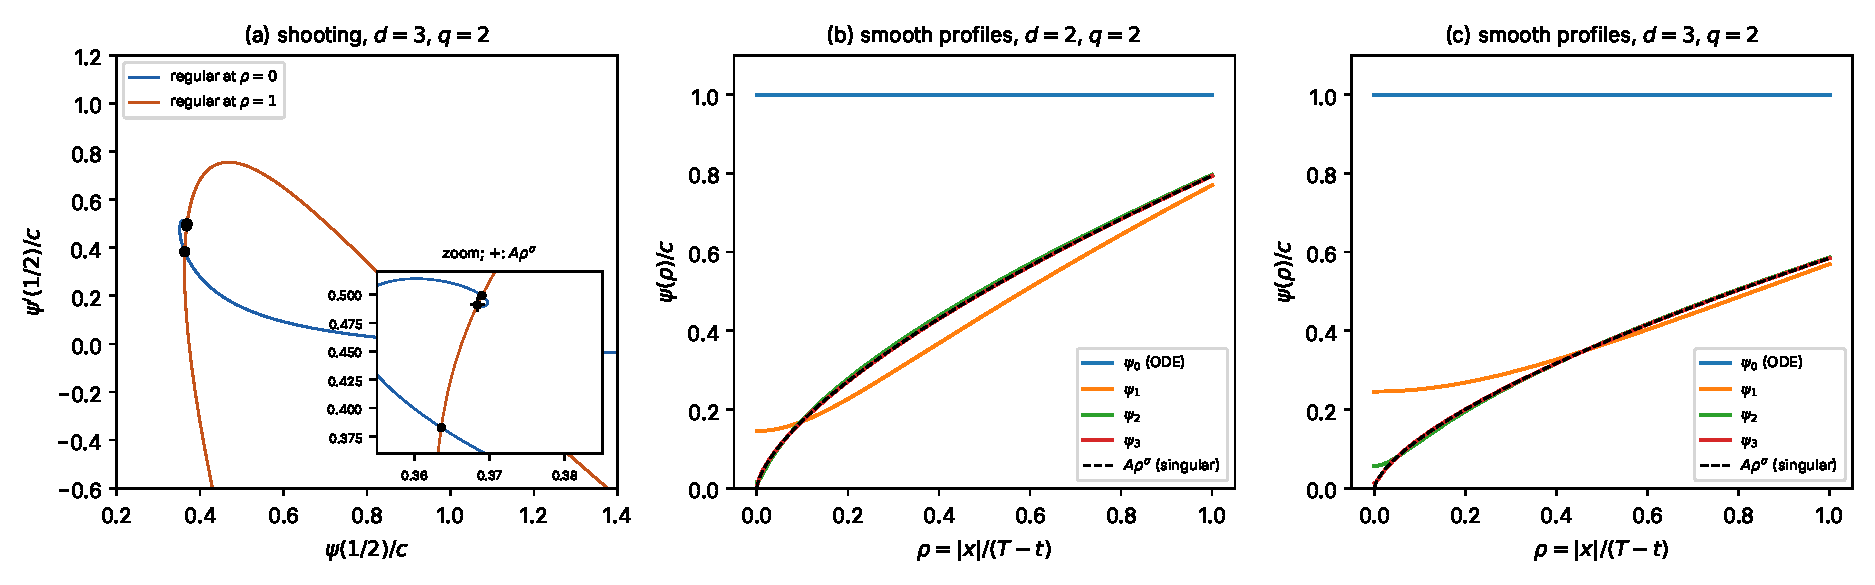
\includegraphics[width=\textwidth]{figures/mems_profile_shooting.pdf}
\caption{(a) Two-sided shooting for $d=3$, $q=2$: the curves of solutions regular
at $\rho=0$ (blue, parametrised by $\psi(0)$) and at $\rho=1$ (orange,
parametrised by $\psi(1)$) in the phase plane at $\rho=\frac12$; intersections
are smooth profiles. The inset shows the spiral of the blue curve around the
singular solution $A\rho^\sigma$. (b), (c) The profiles
$\psi_0\equiv c,\psi_1,\psi_2,\psi_3$ for $d=2,3$, $q=2$, and $A\rho^\sigma$.}
\label{mems:fig-prof}
\end{figure}

\begin{conjecture}\label{mems:conj-prof}
For $d\in\{2,3\}$ and every $q>1$ (more generally whenever $\nu^2>0$),
\eqref{mems:profile-rad} has infinitely many smooth positive solutions
$\psi_n$. They are increasing in $\rho$, and $\psi_n\to\psi_*$ locally
uniformly on $(0,1]$ with $\psi_n(0)/\psi_{n+1}(0)\to e^{\sigma\pi/\nu}$. The
profile $\psi_n$ has exactly $n$ unstable eigenvalues besides those generated by
the symmetries, i.e.\ time and space translations and Lorentz boosts
(\cref{mems:sec-num}). For $d=1$ there are none
(\cref{mems:thm-d1}).
\end{conjecture}

For focusing power nonlinearities, countable families of smooth self-similar
profiles are known \cite{BizonMaisonWasserman2007}, and a proof of
\cref{mems:conj-prof} would presumably follow the same shooting and oscillation
argument. Every $\psi_n$ touches down at the tip with the \emph{same rate}
$(T-t)^{\sigma}$ but a \emph{smaller constant}, $w(t,0)=\psi_n(0)(T-t)^\sigma$
with $\psi_n(0)<c$; the profile is focused at the centre instead of flat.

\subsection{Similarity variables and the free operator}
\label{mems:sec-lin}
With $\psi_1=(T-t)^{-\sigma}w$, $\psi_2=(T-t)^{1-\sigma}\partial_tw$, $T-t=Te^{-\tau}$
(\cref{fw:sec} with $s=-\sigma$), \eqref{mems:eq} becomes
\begin{equation}\label{mems:system}
\partial_\tau\psi_1=-\Lambda\psi_1+\sigma\psi_1+\psi_2,\qquad
\partial_\tau\psi_2=\Delta\psi_1-\Lambda\psi_2-(1-\sigma)\psi_2-\lambda\psi_1^{-q}-\gamma Te^{-\tau}\psi_2 .
\end{equation}
For $\gamma=0$ the static solutions include $\Psi_a=(\psi_a,\Lambda\psi_a-\sigma\psi_a)$, and
$\Psi_0=(c,-\sigma c)$. Writing $\Psi=\Psi_0+\Phi$,
\begin{equation}\label{mems:pert}
  \partial_\tau\Phi=\mathbf L\Phi+\mathbf N(\Phi),\quad
  \mathbf L=\mathbf L_0+\mathbf L',\quad \mathbf L'\Phi=(0,V_0\phi_1),\quad
  \mathbf N(\Phi)=(0,N(\phi_1)),
\end{equation}
where $\mathbf L_0=\mathbf L_0^{(-\sigma)}$ is the free operator of \eqref{fw:system} and
\begin{equation}\label{mems:V0N}
  V_0=q\lambda c^{-q-1}=q\sigma(1-\sigma)=\frac{2q(q-1)}{(q+1)^2},\qquad
  N(\phi)=-\lambda\big[(c+\phi)^{-q}-c^{-q}+qc^{-q-1}\phi\big].
\end{equation}
We work in $\mathcal H^k:=H^k(B^d)\times H^{k-1}(B^d)$, $k\ge2$, and set
$\omega_k:=k-\frac d2-\sigma$. The free operator is \emph{not} dissipative on
low frequencies: polynomial free waves give eigenvalues $\sigma-m$, $m\in\mathbb
N_0$, of $\mathbf L_0$ (e.g.\ $w\equiv1$ gives $(1,0)$ with eigenvalue $\sigma>0$).
The following lemma shows that this is a finite-rank effect. It is a soft
version of the inner-product constructions of
\cite{Ostermann2024,Glogic2025}.

\begin{lemma}[Free operator]\label{mems:lem-free}
Let $k\ge2$ with $\omega_k>0$. There is an inner product $\langle\cdot,\cdot\rangle$
on $\mathcal H^k$, equivalent to the standard one, such that for every
$\varepsilon\in(0,\omega_k)$ there is a finite-rank operator $\mathbf K_\varepsilon$
for which $\mathbf L_0-\mathbf K_\varepsilon$ generates a $C_0$-semigroup with
$\|e^{\tau(\mathbf L_0-\mathbf K_\varepsilon)}\|\le e^{-(\omega_k-\varepsilon)\tau}$.
\end{lemma}

\begin{proof}
\emph{Generation.} For $f\in\mathcal H^k$ extend $f$ to $\mathbb R^d$ (Sobolev
extension), solve the free wave equation and transform back. By finite speed
of propagation this defines a $C_0$-semigroup on $\mathcal H^k$, independent of
the extension, whose generator is the closure of $\mathbf L_0$ on
$C^\infty(\overline{B^d})^2$ (as in
\cite{DonningerSchoerkhuber2017,Ostermann2024}).

\emph{Top order.} For $|\alpha|=k-1$ put $u=\partial^\alpha f$. Since
$[\partial_i,\Lambda]=\partial_i$, $\partial^\alpha\mathbf L_0f$ is the free operator
with $s=-\sigma$ replaced by $s'=-\sigma+k-1$ applied to $u$. Integration by
parts (using $\operatorname{Re}\int_B\nabla u_1\cdot\overline{\nabla\Lambda u_1}=(1-\frac d2)\|\nabla
u_1\|^2+\frac12\int_{\mathbb S^{d-1}}|\nabla u_1|^2$, the analogous identity for
$u_2$, and $\int_B(\nabla u_1\cdot\nabla\bar u_2+\bar u_2\Delta u_1)=\int_{\mathbb S^{d-1}}\bar u_2\,\partial_ru_1$) gives, with $\|f\|_{\dot{\mathcal H}}^2:=\sum_{|\alpha|=k-1}(\|\nabla\partial^\alpha f_1\|^2_{L^2(B)}+\|\partial^\alpha f_2\|^2_{L^2(B)})$,
\begin{equation}\label{mems:energy}
\operatorname{Re}(\mathbf L_0f,f)_{\dot{\mathcal H}}
=-\omega_k\|f\|_{\dot{\mathcal H}}^2-\frac12\sum_{|\alpha|=k-1}\int_{\mathbb S^{d-1}}
\big(|\nabla_{\!T}\partial^\alpha f_1|^2+|\partial_r\partial^\alpha f_1-\partial^\alpha f_2|^2\big)\,dS
\le-\omega_k\|f\|^2_{\dot{\mathcal H}}
\end{equation}
for $f\in C^\infty(\overline{B^d})^2$ ($\nabla_T$ is the tangential gradient). This
is the rigorous form of the heuristic decay rate of \cref{fw:subsec-steps}.

\emph{Low order.} Let $\langle f,g\rangle:=(f,g)_{\dot{\mathcal H}}+(f,g)_{\mathcal
H^{k-1}}$, with $\mathcal H^{k-1}=H^{k-1}\times H^{k-2}$; this is equivalent to
the standard inner product. Since $\mathbf L_0:\mathcal H^k\to\mathcal H^{k-1}$ is
bounded, \eqref{mems:energy} gives
$\operatorname{Re}\langle\mathbf L_0f,f\rangle\le-\omega_k\|f\|^2+C\|f\|\,\|f\|_{\mathcal H^{k-1}}$.
The embedding $J:\mathcal H^k\hookrightarrow\mathcal H^{k-1}$ is compact (Rellich).
So for $\varepsilon>0$ there is a finite-rank orthogonal projection $Q$ in
$\mathcal H^k$ (spectral projection of $J^*J$) with $\|J(I-Q)\|\le\varepsilon/(2C)$.
Then $\|f\|_{\mathcal H^{k-1}}\le\frac{\varepsilon}{2C}\|f\|+\|J\|\|Qf\|$, and
$\operatorname{Re}\langle\mathbf L_0f,f\rangle\le-(\omega_k-\varepsilon)\|f\|^2+C_\varepsilon\|Qf\|^2$.
With $\mathbf K_\varepsilon:=C_\varepsilon Q$, the operator $\mathbf L_0-\mathbf K_\varepsilon+(\omega_k-\varepsilon)$
is dissipative on a core. It is a bounded perturbation of a generator, so
Lumer--Phillips gives the bound \cite[Ch.~II--III]{EngelNagel2000}.
\end{proof}

Since $\mathbf L'$ maps $\mathcal H^k$ into $\{0\}\times H^k\hookrightarrow\{0\}\times H^{k-1}$
compactly, $\mathbf L=(\mathbf L_0-\mathbf K_\varepsilon)+(\mathbf K_\varepsilon+\mathbf L')$
generates a semigroup $\mathbf S(\tau)$, and
$\sigma(\mathbf L)\cap\{\operatorname{Re}\mu>-\omega_k\}$ consists of isolated
eigenvalues of finite algebraic multiplicity (analytic Fredholm theorem;
\cite[IV.5]{Kato1995}, \cite{EngelNagel2000}). In particular the positive free
eigenvalue $\sigma$ is harmless: it is not an eigenvalue of $\mathbf L$.

\subsection{Spectral analysis}
\label{mems:sec-spec}

\begin{proposition}[Spectrum]\label{mems:prop-spec}
Let $k\ge2$ with $\omega_k>0$. A number $\mu$ with $\operatorname{Re}\mu>-\omega_k$ is an
eigenvalue of $\mathbf L$ on $\mathcal H^k$ iff
\begin{equation}\label{mems:eigs}
  \mu\in\{\,1-\ell-2n\,\}\ \cup\ \{\,-(2-2\sigma)-\ell-2n\,\},\qquad \ell,n\in\mathbb N_0,
\end{equation}
($\ell\in\{0,1\}$, the parity, if $d=1$). The eigenfunctions are
$f=(g,(\mu-\sigma+\Lambda)g)$ with $g=|\xi|^\ell Y_\ell(\xi/|\xi|)\,p(|\xi|^2)$,
where $Y_\ell$ is a spherical harmonic and $p$ is a polynomial. The
non-negative eigenvalues are
\begin{itemize}[nosep]
\item $\mu=1$ ($\ell=0$): $f_T=(1,1-\sigma)$, the time-translation mode,
  $\partial_T$ of the rescaled $w^{T,0}$;
\item $\mu=0$ ($\ell=1$, $d$-fold): $f_{L,j}=(\xi_j,(1-\sigma)\xi_j)=(c\sigma)^{-1}\partial_{a_j}\Psi_a|_{a=0}$,
  the Lorentz modes.
\end{itemize}
The largest negative eigenvalues are $\mu=-(2-2\sigma)$ ($\ell=0$, $f_E=(1,\sigma-2)$,
the \emph{energy mode}: the change of $E$ in \cref{mems:prop-ode}(i)) and $\mu=-1$
($\ell=0,n=1$ and $\ell=2,n=0$). Hence the spectral gap is
\begin{equation}\label{mems:gap}
  \omega_0=\min\Big\{1,\ \frac{2(q-1)}{q+1}\Big\}:\qquad
  \omega_0=\tfrac23\ (q=2),\qquad \omega_0=1\ (q\ge3).
\end{equation}
\end{proposition}

\begin{proof}
This is \cref{fw:thm-spec} with $s=-\sigma$; we record the MEMS-specific
points (all identities verified in \texttt{mems\_symbolic\_checks.py}). The
first component of $(\mu-\mathbf L)f=0$ gives $f_2=(\mu-\sigma+\Lambda)f_1$. Then
$f_1=g$ solves \eqref{fw:eig} with $a=\mu-\sigma$, whose characteristic roots
are $a_1=1-\sigma$, $a_2=\sigma-2$ (indeed $1+4V_0=(\frac{3q-1}{q+1})^2$). By interior
elliptic regularity $g\in C^\infty(B^d)$. Its projections
$G_{\ell m}(r)=\int_{\mathbb S^{d-1}}g(r\omega)\overline{Y_{\ell m}(\omega)}d\omega$ lie in
$H^k(\frac12,1)$ and are $O(r^\ell)$ at $0$, hence $G_{\ell m}=\mathrm{const}\cdot
r^\ell{}_2F_1(\alpha,\beta;\ell+\frac d2;r^2)$ with
$\alpha=\frac{\mu-1+\ell}{2}$, $\beta=\frac{\mu+2-2\sigma+\ell}{2}$. (For $d=1$ the
second solution at $0$ has the opposite parity.) At $z=1$ the exponents are
$0$ and $\delta(\mu)=\frac{d-1}2+\sigma-\mu$, and
$\operatorname{Re}\mu>-\omega_k\iff\operatorname{Re}\delta<k-\frac12$. Hence
$(1-z)^{\delta}$ ($\delta\notin\mathbb Z$), $(1-z)^{m}\log(1-z)$ ($\delta=m\in\mathbb N_0$)
and $(1-z)^{-m}$ ($\delta=-m<0$) are not in $H^k$ near $z=1$. In all three
cases the coefficient of the offending term in the connection formula
\cite[15.8]{DLMF} is a nonzero multiple of $1/(\Gamma(\alpha)\Gamma(\beta))$.
Therefore $\alpha\in-\mathbb N_0$ or $\beta\in-\mathbb N_0$, and conversely these
give polynomial (hence admissible) eigenfunctions. The possibility that
\emph{both} Frobenius solutions at $z=1$ are smooth arises only for
$\delta=m\in\mathbb N$ with $(\alpha)_m(\beta)_m=0$, which is again covered by
$\alpha$ or $\beta\in-\mathbb N_0$. Since the solution regular at $0$ is
unique up to a factor, each harmonic $Y_{\ell m}$ contributes at most one
eigenfunction. The two families overlap only if $\alpha-\beta=\sigma-\frac32\in\mathbb Z$,
i.e.\ for $q=3$ (\cref{mems:rem-q3}). Solving $\alpha=-n$, $\beta=-n$ gives \eqref{mems:eigs}. The physical
identification follows from \cref{mems:lem-sym}, and from the spatially
homogeneous perturbations $(T-t)^{\sigma-1}$ and $(T-t)^{2-\sigma}$ of the ODE
(roots of $m(m-1)=V_0$), which correspond to $\mu=1$ and $\mu=-(2-2\sigma)$.
\end{proof}

\begin{lemma}[Semisimplicity]\label{mems:lem-jordan}
Let $d\le3$ and let $k\ge2$ with $\omega_k>0$. Then $(1-\mathbf L)g=f_T$ and
$(-\mathbf L)g=f_{L,j}$ have no solution $g\in\mathcal D(\mathbf L)$. Consequently the
Riesz projections $\mathbf P_1$ (at $\mu=1$) and $\mathbf P_0$ (at $\mu=0$) have
ranks $1$ and $d$, with $\operatorname{ran}\mathbf P_1=\langle f_T\rangle$ and
$\operatorname{ran}\mathbf P_0=\langle f_{L,1},\dots,f_{L,d}\rangle$.
\end{lemma}

\begin{proof}
$(\mu-\mathbf L)g=f$ is equivalent to $g_2=(a+\Lambda)g_1-f_1$ and
$-\big[(\delta_{ij}-\xi_i\xi_j)\partial_{ij}g_1-2(a+1)\Lambda g_1-(a(a+1)-V_0)g_1\big]=f_2+(a+1)f_1+\Lambda f_1$.
For $f=f_T$ ($a=1-\sigma$, so $a(a+1)=V_0$) the right side is $3-2\sigma$; for
$f=f_{L,j}$ ($a=-\sigma$) it is $(3-2\sigma)\xi_j$. With $g_1=G(r)$, resp.\
$g_1=rK(r)\xi_j/|\xi|$, both reduce to the first-order equation
\[
  (1-r^2)P'+\Big(\frac{D-1}{r}-2(2-\sigma)r\Big)P=-(3-2\sigma),\qquad P=G'\ (D=d),\quad P=K'\ (D=d+2).
\]
The solution regular at $r=0$ is
$P=-(3-2\sigma)r^{1-D}(1-r^2)^{-(e+1)}\int_0^r s^{D-1}(1-s^2)^{e}ds$ with
$e=\frac{3-D}2-\sigma$. Near $r=1$,
$\int_0^r s^{D-1}(1-s^2)^e\,ds=C_D+(1-r^2)^{e+1}A(r)$ with $A$ analytic and
\[
  C_D=\frac{\Gamma(\frac D2)\,\Gamma(e+1)}{2\,\Gamma(\frac52-\sigma)}\neq0
\]
(analytic continuation of the Beta integral when $e<-1$). The only exception
is $e+1\in-\mathbb N_0$, which for $d\le3$ happens only for $D=4$, $q=3$, where a
term $\log(1-r^2)$ with coefficient $-\frac12$ appears instead. Hence $g_1$
contains $C\,(1-r)^{\delta(\mu)}$ with $C\ne0$ and $\delta(1)=\frac{d-3}2+\sigma$,
$\delta(0)=\frac{d-1}2+\sigma$. Both are non-integers for $d\le3$, except for
$(d,q)=(2,3)$, where $\delta(1)=0$ and $\delta(0)=1$ and one gets $\log(1-r)$,
resp.\ $(1-r)\log(1-r)$, instead. As
$\delta(\mu)<k-\frac12$, $g_1\notin H^k$. (The constant $C_D$ and the expansion
were checked numerically with \texttt{mpmath}.)
\end{proof}

\begin{remark}[$q=3$: a Jordan block at the gap]\label{mems:rem-q3}
For $q=3$ the two families in \eqref{mems:eigs} collide at $\mu=-1=-\omega_0$ in the
sector $\ell=0$, with the single eigenfunction $f_E=(1,-\frac32)$. In this case
$(-1-\mathbf L)g=f_E$ \emph{is} solvable with
$g=(|\xi|^2/d,\ |\xi|^2/(2d)-1)$, so $\mu=-1$ carries a Jordan block (verified
symbolically; in the collocation of \cref{mems:sec-num} this double eigenvalue
splits by $\approx10^{-5}$, much more than the errors for simple eigenvalues). Hence for van der Waals forces the decay at the
rate $\omega_0=1$ fails by a factor $\tau$, which matches the $\theta\log\theta$
term in \eqref{mems:dampedexp} below. This does not affect
\cref{mems:thm-main}, where $\omega<\omega_0$.
\end{remark}

\begin{proposition}[Linear stability]\label{mems:prop-lin}
Let $d\le3$, $k\ge2$, $\omega_k>0$, and $\mathbf P=\mathbf P_1+\mathbf P_0$. Then
$\mathbf S(\tau)\mathbf P_1=e^\tau\mathbf P_1$, $\mathbf S(\tau)\mathbf P_0=\mathbf P_0$, and for every
$\omega<\min\{\omega_0,\omega_k\}$ there is $M_\omega$ with
$\|\mathbf S(\tau)(\mathbf I-\mathbf P)f\|\le M_\omega e^{-\omega\tau}\|(\mathbf I-\mathbf P)f\|$.
\end{proposition}

\begin{proof}
Fix $\omega<\omega'<\min\{\omega_0,\omega_k-\varepsilon\}$. On $\operatorname{Re}\mu\ge-\omega'$,
$\mathbf R_{\mathbf L}(\mu)=\mathbf R_0(\mu)[\mathbf I-(\mathbf K_\varepsilon+\mathbf L')\mathbf R_0(\mu)]^{-1}$ with
$\mathbf R_0$ the resolvent of $\mathbf L_0-\mathbf K_\varepsilon$. Here
$\|\mathbf L'\mathbf R_0(\mu)\|\lesssim|\mu|^{-1}$. Indeed, $u=\mathbf R_0(\mu)f$
satisfies $\mu u_1=f_1-\Lambda u_1+\sigma u_1+u_2+(\mathbf K_\varepsilon u)_1$, so
$\|u_1\|_{H^{k-1}}\lesssim|\mu|^{-1}\|f\|$. Also
$\|\mathbf K_\varepsilon\mathbf R_0(\mu)\|\to0$ as $|\mu|\to\infty$: write $\mathbf K_\varepsilon$
via vectors in the dense set $\mathcal D(\mathbf L_0^*)$, up to a small error.
Hence $\mathbf R_{\mathbf L}$ is uniformly bounded for $|\mu|$ large. On the
remaining compact set it is analytic except at $\mu=1,0$
(\cref{mems:prop-spec}). The Gearhart--Prüss theorem
\cite[V.1.11]{EngelNagel2000} applied to $\mathbf L|_{\operatorname{ran}(\mathbf I-\mathbf P)}$
gives the bound. \Cref{mems:lem-jordan} gives the action on $\operatorname{ran}\mathbf P$.
\end{proof}

\paragraph{Required regularity.} To see the full gap one needs $\omega_k\ge\omega_0$,
i.e.\ $k\ge\frac d2+\sigma+\omega_0$, together with $k>\frac d2$ (for the
nonlinearity) and $k\ge2$. Since $\sigma+\omega_0=\min\{1+\sigma,2-\sigma\}\le\frac32$,
\[
  k=2\ (d=1),\qquad k=3\ (d=2,3)\qquad\text{suffice for every }q>1 .
\]
For $(d,q)=(1,3),(3,3)$ the value $\omega_k=\omega_0=1$ is attained exactly, which is
harmless since $\omega<\omega_0$. For smaller admissible $k$ (e.g.\ $k=2$, $d=2$) everything
holds with $\omega<\min\{\omega_0,\omega_k\}$.

\subsection{Nonlinear stability of ODE touchdown}
\label{mems:sec-nonlin}
Normalise $T_0=1$ by scaling. The reference solution $w^{1,0}=c(1-t)^\sigma$ has
data $(c,-\sigma c)$ at $t=0$.

\begin{theorem}[Stable self-similar touchdown]\label{mems:thm-main}
Let $\gamma=0$, $q>1$, $\lambda>0$, $d\in\{1,2,3\}$, $k=2$ if $d=1$ and $k=3$ if
$d=2,3$, and $0<\omega<\omega_0=\min\{1,\frac{2(q-1)}{q+1}\}$. There are
$\delta>0$, $M\ge1$ such that the following holds. Let real data
$(w_0,w_1)=(c,-\sigma c)+(v_0,v_1)$ satisfy
$\|(v_0,v_1)\|_{H^k\times H^{k-1}(B_{1+\delta})}\le\delta/M$. Then there exist
$T^*\in[1-\delta,1+\delta]$ and $a^*\in\mathbb R^d$, $|a^*|\le\delta$, such that the
solution $w$ of \eqref{mems:eq} with these data exists in the backward cone
$\Gamma_{T^*}$, is positive there, touches down at $(T^*,0)$, and satisfies, for
$0\le t<T^*$,
\begin{align*}
  (T^*-t)^{|\alpha|-\sigma-\frac d2}\big\|\partial_x^\alpha\big(w(t)-w^{T^*,a^*}(t)\big)\big\|_{L^2(B_{T^*-t})}&\lesssim\delta\,(T^*-t)^{\omega},\quad|\alpha|\le k,\\
  (T^*-t)^{|\alpha|+1-\sigma-\frac d2}\big\|\partial_x^\alpha\partial_t\big(w(t)-w^{T^*,a^*}(t)\big)\big\|_{L^2(B_{T^*-t})}&\lesssim\delta\,(T^*-t)^{\omega},\quad|\alpha|\le k-1.
\end{align*}
In particular, uniformly for $|x|\le T^*-t$,
\begin{gather*}
  w(t,x)=(T^*-t)^{\sigma}\Big[\psi_{a^*}\Big(\frac{x}{T^*-t}\Big)+O\big(\delta(T^*-t)^{\omega}\big)\Big],\\
  \partial_tw(t,0)=-\sigma c\,(1-|a^*|^2)^{-\frac\sigma2}(T^*-t)^{\sigma-1}\big(1+O((T^*-t)^{\omega})\big).
\end{gather*}
If the data are radial (even, if $d=1$), then $a^*=0$.
\end{theorem}

\begin{proof}[Proof sketch]
\emph{1. Data and unknowns.} For $T\in[1-\delta,1+\delta]$ and $|a|\le\delta$, the
rescaled data are $\mathbf U(v,T)=(T^{-\sigma}w_0(T\cdot),T^{1-\sigma}w_1(T\cdot))$ on
$B^d$ ($B_T\subset B_{1+\delta}$). We write $\Psi(\tau)=\Psi_a+\Phi(\tau)$, so that
$\Phi(0)=\mathbf u(T,a):=\mathbf U(v,T)-\Psi_a$ and
\[
  \partial_\tau\Phi=\mathbf L\Phi+\mathbf G_a(\Phi),\qquad
  \mathbf G_a(\Phi)=\big(0,\ (V_a-V_0)\phi_1+N_a(\phi_1)\big),
\]
with $V_a=q\lambda\psi_a^{-q-1}$, $\|V_a-V_0\|_{C^k(\overline B)}\lesssim|a|$,
and $N_a(\phi)=-\lambda[(\psi_a+\phi)^{-q}-\psi_a^{-q}+q\psi_a^{-q-1}\phi]$.

\emph{2. Nonlinearity.} As $k>\frac d2$, $H^k(B^d)$ is an algebra and
$\|\phi\|_{L^\infty}\le C_k\|\phi\|_{H^k}$. For $\|\phi\|_{H^k}\le\delta$ with $C_k\delta\le c/4$
we have $\psi_a+\phi\ge c/4$ on $\overline{B^d}$, i.e.\ the solution stays away from
the singularity of $w^{-q}$, and $N_a(\phi)=\phi^2\int_0^1(1-\theta)F''(\psi_a+\theta\phi)\,d\theta$ with
$F(w)=-\lambda w^{-q}$ smooth on $[c/4,\infty)$. Moser estimates give
$\|N_a(\phi)-N_a(\tilde\phi)\|_{H^{k-1}}\lesssim(\|\phi\|_{H^k}+\|\tilde\phi\|_{H^k})\|\phi-\tilde\phi\|_{H^k}$.

\emph{3. Modified Duhamel equation.} In
$\mathcal X=\{\Phi\in C([0,\infty),\mathcal H^k):\|\Phi\|_{\mathcal X}:=\sup_\tau e^{\omega\tau}\|\Phi(\tau)\|\le\delta\}$ solve
\begin{gather*}
  \Phi(\tau)=\mathbf S(\tau)\big[\mathbf u-\mathbf C(\Phi,\mathbf u)\big]+\int_0^\tau\mathbf S(\tau-\tau')\mathbf G_a(\Phi(\tau'))\,d\tau',\\
  \mathbf C(\Phi,\mathbf u)=\mathbf P\mathbf u+\int_0^\infty\big(e^{-\tau'}\mathbf P_1+\mathbf P_0\big)\mathbf G_a(\Phi(\tau'))\,d\tau'.
\end{gather*}
By Step 2, $\|\mathbf G_a(\Phi)(\tau)\|\lesssim(\delta^2+|a|\delta)e^{-\omega\tau}$, with the
corresponding Lipschitz bound. By \cref{mems:prop-lin}, the
right-hand side maps $\mathcal X$ into itself and is a contraction, provided
$\|(\mathbf I-\mathbf P)\mathbf u\|\le\delta/(2M_\omega)$. This holds because
$\mathbf u(T,a)=[\mathbf U(0,T)-\Psi_0]+[\Psi_0-\Psi_a]+[\mathbf U(v,T)-\mathbf U(0,T)]$, with
\[
  \mathbf U(0,T)-\Psi_0=-c\sigma(T-1)f_T+O((T-1)^2),\qquad
  \Psi_0-\Psi_a=-c\sigma\,a\cdot f_L+O(|a|^2),
\]
so $\|(\mathbf I-\mathbf P)\mathbf u\|\lesssim\delta/M+\delta^2$. The fixed point $\Phi_{T,a}$ is
continuous in $(T,a)$.

\emph{4. Choice of $(T^*,a^*)$.} In the basis $f_T,f_{L,1},\dots,f_{L,d}$ of
$\operatorname{ran}\mathbf P$,
$\mathbf C(\Phi_{T,a},\mathbf u(T,a))=-c\sigma\big((T-1)f_T+a\cdot f_L\big)+\mathbf R(T,a)$ with
$\mathbf R$ continuous and $|\mathbf R|\lesssim\delta/M+\delta^2$. (The terms are
exactly the symmetry generators, \cref{mems:prop-spec}.) By Brouwer's fixed
point theorem there is $(T^*,a^*)\in[1-\delta,1+\delta]\times\overline{B_\delta}$ with
$\mathbf C=0$, for $M$ large and $\delta$ small. Then $\Phi$ solves the true Duhamel
equation. For radial data everything can be done in the radial subspace,
where $\mathbf P_0=0$, so $a^*=0$.

\emph{5. Back to $w$.} The mild solution coincides with the (strong) solution of
\eqref{mems:eq} in $\Gamma_{T^*}$ (approximation by smooth data and finite
speed of propagation). Since $\psi_1=\psi_{a^*}+\phi_1$ and
$\|\phi_1(\tau)\|_{L^\infty}\lesssim\delta e^{-\omega\tau}$, $w>0$ in the cone and $w(t,0)\to0$.
The estimates are $\|\Phi(\tau)\|_{\mathcal H^k}\le\delta e^{-\omega\tau}$ rewritten
with $e^{-\tau}=(T^*-t)/T^*$. The formula for $\partial_tw(t,0)$ uses
$H^{k-1}\hookrightarrow C^0$, which holds since $k-1>\frac d2$ for our
choices of $k$.
\end{proof}

\begin{remark}\label{mems:rem-main}
(a) \emph{No translation parameter is needed.} The ODE profile is
translation invariant, and $w^{T,a}(\cdot,\cdot-x_0)=w^{T-a\cdot x_0,a}$. Applying
the theorem at every nearby base point $x_0$ (translated data) shows that,
near $x_0=0$, touchdown happens along a hypersurface $t=T^*(x_0)$. For the
exact solutions $a=\nabla T^*$. We expect $a^*=\nabla T^*(0)$ and $T^*\in C^1$
in general, as for the 1D power case \cite{MerleZaag2007}; we have not proved it.
(b) The rate $\omega_0=\frac23$ for $q=2$ is dictated by the ODE energy mode
$\mu=-(2-2\sigma)$. For $q\ge3$ it is the PDE mode $\mu=-1$, which by
\cref{mems:rem-q3} is not semisimple when $q=3$.
(c) The theorem is in the style of
\cite{DonningerSchoerkhuber2016,DonningerSchoerkhuber2017,Ostermann2024}.
The new features are $s<0$ (\cref{mems:lem-free}) and the need to keep the
solution away from $w=0$, which the $L^\infty$ control from $k>\frac d2$
provides.
\end{remark}

\subsection{Damping and other integrable perturbations}
\label{mems:sec-damp}
In \eqref{mems:system}, damping contributes $-\gamma Te^{-\tau}\psi_2$, a perturbation
decaying at rate $1\ge\omega_0$. Exact self-similar solutions no longer exist
(there is no scaling symmetry), but the touchdown remains asymptotically
self-similar.

\paragraph{Damped ODE.} For $W''+\gamma W'=-\lambda W^{-q}$, inserting
$W=c\theta^\sigma(1+c_1\theta+\dots)$, $\theta=T-t$, the $\theta^{\sigma-1}$-terms give
$c_1\sigma(3-q)=\gamma\sigma$. Including the free energy mode,
\begin{equation}\label{mems:dampedexp}
  W=c\,\theta^\sigma\Big(1+e\,\theta^{2-2\sigma}+\frac{\gamma}{3-q}\,\theta+\dots\Big)\ (q\ne3),\qquad
  W=c\,\theta^{1/2}\Big(1+\frac{\gamma}{4}\,\theta\log\theta+e\,\theta+\dots\Big)\ (q=3).
\end{equation}
For $q=2$, $c_1=\gamma$. For $q<3$ the damping correction is positive (larger gap at
the same remaining time and the same $e$); for $q>3$ it is negative. For $q=3$ the exponents $1$ and $2-2\sigma$ resonate. Both formulas are
confirmed numerically (fitted coefficients within $0.4\%$ of the predicted ones;
\texttt{mems\_damped\_ode.py}). In
similarity variables the background is $\Psi_0+O(\gamma Te^{-\tau})$ (or
$O(\gamma T\tau e^{-\tau})$ if $q=3$).

\begin{proposition}[Damped touchdown, sketch]\label{mems:prop-damped}
Assume the hypotheses of \cref{mems:thm-main}, except that the damping
satisfies $0\le\gamma\le\delta/M$, i.e.\ $\gamma T_0\le\delta/M$ in general units.
Then the conclusions of \cref{mems:thm-main} hold verbatim, for radial and
nonradial data, with the same comparison profiles $w^{T^*,a^*}$.
\end{proposition}

\begin{proof}[Sketch]
Add $-\gamma Te^{-\tau}(0,\psi_{a,2}+\phi_2)$ to $\mathbf G_a$. Its size is
$\lesssim\gamma e^{-\tau}\le\gamma e^{-\omega\tau}$, its Lipschitz constant is $\lesssim\gamma$, and
$\int_0^\tau e^{-\omega'(\tau-\tau')}e^{-\tau'}d\tau'\lesssim e^{-\omega\tau}$ since $\omega<\omega'<\omega_0\le1$.
Steps 3--5 go through with $\delta^2+|a|\delta$ replaced by
$\delta^2+|a|\delta+\gamma$. The key point for the nonradial case is that the
neutral component obeys $\frac{d}{d\tau}\mathbf P_0\Phi=\mathbf P_0\mathbf G_a(\Phi)$
(no Jordan block). The right side is \emph{integrable} in $\tau$, so
$\mathbf P_0\Phi(\tau)$ has a limit, and the static choice of $a$ by Brouwer makes it
zero. A dynamical modulation of the boost (cf.\ \cref{fw:subsec-lower}) would
be needed only for a non-integrable forcing of the neutral modes.
\end{proof}

\begin{corollary}[Arbitrary damping; sketch]\label{mems:cor-damped}
Let $\gamma\ge0$ and let $W$ be any solution of the damped ODE that touches down at
$T_0>0$. Then data close enough to $(W(0),W'(0))$ in
$H^k\times H^{k-1}(B_{T_0+\eta})$ lead to touchdown at $(T^*,0)$, $T^*\to T_0$ as
the data converge, with the asymptotics of \cref{mems:thm-main}.
\end{corollary}

\begin{proof}[Sketch]
By \eqref{mems:dampedexp}, at $t_1=T_0-\theta_1$ the rescaled data of $W$ differ
from $(c,-\sigma c)$ by $O(\theta_1^{\min\{1,2-2\sigma\}})$ (times $\log$ if $q=3$), and the
rescaled damping is $\gamma\theta_1$. Choose $\theta_1$ so small that both are
$\le\delta/(2M)$. By local well-posedness and continuous dependence on
$[0,t_1]$ (the solution stays near $W(t)\ge W(t_1)>0$), data close enough to
those of $W$ produce data at $t_1$ satisfying the hypotheses of
\cref{mems:prop-damped} after rescaling by $\theta_1$.
\end{proof}

The same argument covers any perturbation that is $O(e^{-\tau})$ in similarity
variables. For instance a smooth dielectric profile $f(x)>0$ in
$-\lambda f(x)w^{-q}$ gives
$\lambda f(Te^{-\tau}\xi)\psi_1^{-q}=\lambda f(0)\psi_1^{-q}+O(e^{-\tau})$.
Touchdown at a point $x_0$ is then ODE-like with $c=c(\lambda f(x_0))$. This is
not written out.

\subsection{Physical interpretation}
\label{mems:sec-phys}
\begin{itemize}[leftmargin=1.2em]
\item \emph{Rate and impact speed.} For the Coulomb force ($q=2$) the gap
closes like $w\approx(9\lambda/2)^{1/3}(T-t)^{2/3}$, i.e.\
$1+u\approx(9\lambda/2)^{1/3}\big((T-t)/\varepsilon\big)^{2/3}$ in the original time.
The impact speed $u_t\sim-\frac23(9\lambda/2)^{1/3}\varepsilon^{-2/3}(T-t)^{-1/3}$
is infinite. In the parabolic model ($\varepsilon=0$) the ODE
$W'=-\lambda W^{-2}$ gives instead $w\approx(3\lambda(T-t))^{1/3}$; for the
rigorous parabolic theory see \cite{EspositoGhoussoubGuo2010} and references
therein.
% TODO verify and cite Guo--Pan--Ward, SIAM J. Appl. Math. 66 (2005) for the parabolic rate (T-t)^{1/3}.
For $\varepsilon>0$, inertia dominates damping once
$T-t\ll\varepsilon^2/\gamma$ (the scale-invariant damping is $\gamma(T-t)/\varepsilon^2$).
Hence the \emph{final} touchdown asymptotics is the hyperbolic one,
\cref{mems:cor-damped}, and the parabolic rate is at most an intermediate
regime for $\varepsilon^2\ll T-t\ll1$.
\item \emph{Flat profile, touchdown on a hypersurface.} The stable profile is
constant in the light cone. Near touchdown the gap closes uniformly over a
region of size $\sim T-t$ (in units of the wave speed), and the touchdown set
is locally a spacelike hypersurface $t=T^*(x)$
(\cref{mems:rem-main}(a)). This differs sharply from parabolic MEMS, where
touchdown is typically at isolated points. The focused profiles $\psi_n$ of
\cref{mems:conj-prof} touch down at a point but are unstable.
\item \emph{Locality.} Only data in the base of the cone, $B_{T^*}(x_0)$, matter.
The clamped boundary, the shape of $\Omega$ and the far-away dielectric profile are
irrelevant as long as this ball lies inside $\Omega$.
\item \emph{An explicit scenario.} Release the undamped device ($q=2$) from rest,
$w\equiv1$, $w_t\equiv0$, and let $B_R(x_0)\subset\Omega$. By finite speed of
propagation $w(t,x)=W(t)$ for $|x-x_0|<R-t$. If
$T_0=\pi/(2\sqrt{2\lambda})<R$, i.e.\ $\lambda>\pi^2/(8R^2)$, the membrane therefore
touches down \emph{simultaneously on the ball} $|x-x_0|<R-T_0$ (unless it has
quenched elsewhere earlier; we have not excluded this). By
\cref{mems:thm-main,mems:prop-damped} this flat touchdown is stable under
small perturbations of the data, of the damping and of the permittivity. It
then occurs on a nearby spacelike hypersurface with a boosted ODE profile.
For $R=1$ the threshold $\pi^2/8\approx1.234$ should be compared with the
static pull-in values $\lambda^*\approx0.350$ (interval $(-1,1)$), $0.789$ (unit
disk) and $1.299$ (unit ball in $\mathbb R^3$) (\texttt{mems\_damped\_ode.py}).
\item \emph{Dimensions.} $d=1$ describes strings and membrane strips (beams with
bending stiffness, $\Delta^2$, are \emph{not} covered: there is no light cone);
$d=2$ describes the membrane (e.g.\ a disk); $d=3$ is included for comparison
with the wave-equation literature.
\end{itemize}

\subsection{Numerical checks}
\label{mems:sec-num}
The eigenvalue problem in the sector $\ell$ is the quadratic pencil
$z(1-z)h''+(\ell+\frac d2-(b+\frac32)z)h'-\frac14(b^2+b-V)h=0$,
$b=\mu-\sigma+\ell$, $g=|\xi|^\ell Y_\ell h(|\xi|^2)$. We solved it by Chebyshev
collocation in $z\in[0,1]$ without boundary conditions, keeping eigenvalues
that are stable under refinement ($N=20,28$; larger $N$ starts to resolve the
non-smooth generalised eigenfunctions of $\operatorname{Re}\mu\le-\omega_k$ and produces
spurious eigenvalues). For $V\equiv V_0$, $q=2,3,4$, $d=1,2,3$ and
$\ell\le2$, all eigenvalues with $\operatorname{Re}\mu>-1.9$ agree with
\eqref{mems:eigs} to $\le10^{-5}$. No others appear. For $q=3$ the double
eigenvalue $-1$ splits as expected for a Jordan block. An independent
discretisation of the full first-order operator $\mathbf L$ for $d=1$ gives
$\{1,0,-\frac23,-1,-\frac53\}$ for $q=2$ (both parities), as predicted.
For the excited profiles ($d=3$, $q=2$, $V=q\lambda\psi_n^{-q-1}$) we find:
\begin{itemize}[nosep]
\item $\psi_1$: $\{3.4955,\,1\}$ for $\ell=0$; $\{1,\,0\}$ for $\ell=1$ (space
translation, which is non-trivial for a non-constant profile, and boost); none
for $\ell=2$.
\item $\psi_2$: $\{20.35,\,3.598,\,1\}$ for $\ell=0$ (this needs $N\ge120$).
\end{itemize}
Thus $\psi_1$ has one and $\psi_2$ two genuinely unstable directions, as in
\cref{mems:conj-prof}. See \cref{mems:fig-spec}
(\texttt{mems\_spectrum\_numerics.py}). The independent numerics section of this
note provides a further check.

\begin{figure}[ht]
\centering
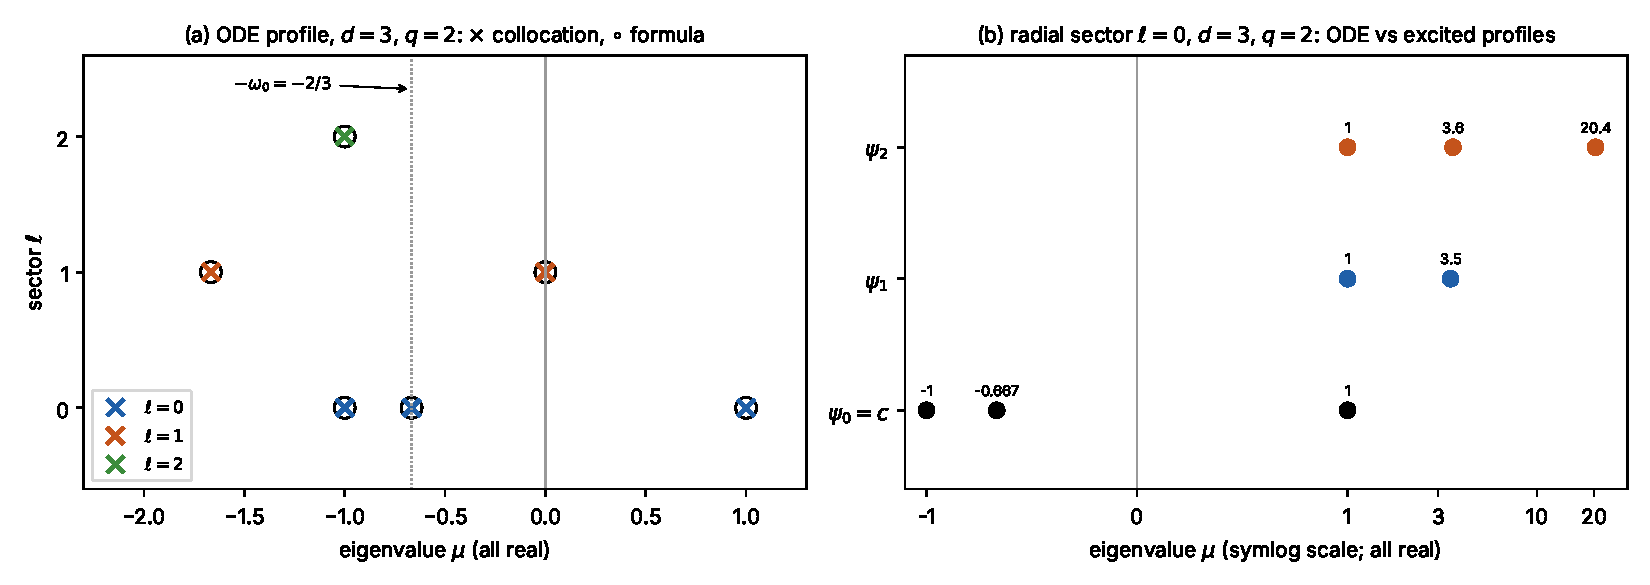
\includegraphics[width=\textwidth]{figures/mems_spectrum.pdf}
\caption{(a) Eigenvalues of the linearisation at the ODE profile, $d=3$, $q=2$,
sectors $\ell=0,1,2$: collocation ($\times$) versus \eqref{mems:eigs} ($\circ$);
the dotted line is $-\omega_0=-\frac23$ (energy mode). (b) Radial eigenvalues
($\operatorname{Re}\mu>-0.3$ for $\psi_{1,2}$) of the ODE profile $\psi_0=c$ and of the
first two excited profiles: $\psi_n$ has $n$ unstable eigenvalues in addition to
the time-translation eigenvalue $1$.}
\label{mems:fig-spec}
\end{figure}

\subsection{Relation to Gimperlein--He--Lacey}
\label{mems:sec-ghl}
The closest prior work is \cite{GimperleinHeLacey2022} (see also
\cite{He2021}). According to the summary in \cref{lit:mems}, it studies the
self-similar quenching of \eqref{lit:eq:memsq} formally and numerically:
\begin{itemize}[nosep]
\item it treats the ODE profile $\kappa_q(T-t)^{2/(q+1)}$;
\item it obtains formally a sequence of self-similar solutions;
\item it gives evidence that radial solutions increasing in $|x|$ quench at the
origin, that the trivial profile is stable up to time translation, and that the
non-trivial ones are unstable.
\end{itemize}
\emph{Caveat: the text of \cite{GimperleinHeLacey2022} could not be consulted
while this section was written (no network access). The points below compare
with that summary only, and should be checked against the paper.}
% TODO (R. He): check the comparison below against arXiv:2210.14821.
\begin{enumerate}[label=(\alph*),nosep]
\item \emph{Profile and constant.} $\kappa_q=c$, with
$c^{q+1}=\lambda(q+1)^2/(2(q-1))$, \eqref{lit:eq:memsode}.
\item \emph{Non-trivial profiles.} Our $\psi_n$
(\cref{mems:tab-prof}) are increasing in $|x|$ and accumulate at the
\emph{static} singular solution $A|x|^{2/(q+1)}$. The ratio law
$\psi_n(0)/\psi_{n+1}(0)\to e^{\sigma\pi/\nu}$ gives a sharp quantitative test for
identifying them with the sequence of \cite{GimperleinHeLacey2022}.
\Cref{mems:thm-d1} shows that the sequence has no counterpart in $d=1$.
\item \emph{Stability.} We make the stability of the ODE profile rigorous:
modulo time translation for radial data and modulo time translation plus
Lorentz boosts in general (\cref{mems:thm-main}), with damping
(\cref{mems:prop-damped,mems:cor-damped}). We also give the decay rate
$(T-t)^{\omega}$, $\omega<\min\{1,\frac{2(q-1)}{q+1}\}$, and identify the slowest
stable mode as the ODE energy mode for $q<3$. The numerically computed extra
unstable eigenvalues of $\psi_1,\psi_2$ support the instability of the
non-trivial profiles.
\end{enumerate}

\subsection{Caveats and open points}
\label{mems:sec-gaps}
\begin{enumerate}[nosep]
\item \Cref{mems:thm-main,mems:prop-damped,mems:cor-damped} are proof sketches.
The standard parts are referenced, not reproduced: generation of
$\mathbf L_0$ on $\mathcal H^k$, equivalence of mild and strong solutions,
continuity of the fixed point in $(T,a)$, and Moser estimates.
\Cref{mems:lem-free,mems:prop-spec,mems:lem-jordan} are complete modulo
routine details. \Cref{mems:lem-jordan} is stated for $d\le3$; the general
case needs the same Beta-function check.
\item The statements are local in the backward cone. Which points touch down
first, the regularity of the touchdown hypersurface, $a^*=\nabla T^*$, and
the behaviour outside the cone are open.
\item The existence of the non-trivial profiles for $d\ge2$ is numerical
(\cref{mems:conj-prof}); their spectra are low-precision numerics.
Nonradial non-trivial profiles were not searched for.
\item For $q=3$ the eigenvalue $-\omega_0$ is a Jordan block
(\cref{mems:rem-q3}), so the rate $\omega_0=1$ itself is not attained.
\item Not covered: plate models with $\Delta^2$, and nonlocal (series
capacitor) models. In the latter the coefficient
$\lambda(1+\alpha\int w^{-1})^{-2}$ depends on the whole solution, and a flat
touchdown on a set of positive measure would drive it to $0$ (heuristic, not
analysed).
\end{enumerate}
